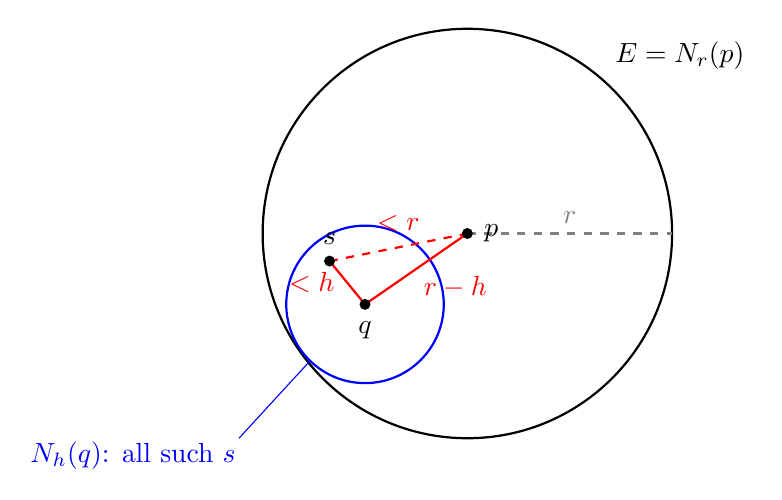
\begin{tikzpicture}[line width=0.8pt, dot/.style={circle, fill, inner sep=1.4pt}]
  \coordinate (p) at (0,0);
  \coordinate (q) at (-1.3,-0.9);
  \coordinate (s) at (-1.75,-0.35);
  % big neighborhood
  \draw (p) circle (2.6);
  \node[anchor=south west] at (1.75,1.95) {$E = N_r(p)$};
  % radius r from p
  \draw[gray, dashed] (p) -- (2.6,0) node[midway, above] {$r$};
  % small neighborhood around q
  \draw[blue] (q) circle (1.0);
  \draw[blue, thin] (-2.0,-1.62) -- (-2.9,-2.6) node[anchor=north east, inner sep=1pt] {$N_h(q)$: all such $s$};
  % triangle
  \draw[red] (q) -- (p) node[midway, below right=-1pt] {$r-h$};
  \draw[red] (q) -- (s) node[midway, left=1pt] {$<h$};
  \draw[red, dashed] (s) -- (p) node[midway, above=2pt] {$<r$};
  \node[dot, label=right:$p$] at (p) {};
  \node[dot, label=below:$q$] at (q) {};
  \node[dot, label=above:$s$] at (s) {};
\end{tikzpicture}
